\documentclass[11pt]{article}

% Typography
\usepackage[utf8]{inputenc}
\usepackage[T1]{fontenc}
\usepackage{mathpazo}               % Palatino for text and math (scalable)
\usepackage[scaled=0.85]{berasans} % Bera Sans for sans-serif
\usepackage[scaled=0.85]{beramono} % Bera Mono for monospace
\usepackage{microtype}             % Better typographic refinement

% Layout
\usepackage[margin=1in]{geometry}
\usepackage{setspace}
\setstretch{1.15}                  % Slightly opened up line spacing
\usepackage{parskip}              % Paragraph spacing instead of indentation

% Math and tables
\usepackage{graphicx}
\usepackage{amsmath}
\usepackage{amssymb}
\usepackage{booktabs}
\usepackage{tabularx}
\usepackage{array}
\usepackage{enumitem}
\usepackage[font=small,labelfont=bf]{caption}

% References
\usepackage{xcolor}
\usepackage[colorlinks,citecolor=blue!60!black,linkcolor=blue!60!black,urlcolor=blue!60!black]{hyperref}
\usepackage[round]{natbib}

\newcolumntype{Y}{>{\raggedright\arraybackslash}X}
\newcommand{\dhh}{\Delta h}
\newcommand{\WU}{W_U}

\title{Contrastive Projection: Reading Transformer Internals\\ by Differencing Logit Lenses}
\author{Olli Tuomi\\ Evident Solutions Oy}
\date{}

\begin{document}
\maketitle

\begin{abstract}
Subtracting the hidden states of two matched inputs at each layer and
projecting through the unembedding matrix $\WU$ produces a training-free,
layer-by-layer readout of what separates them in token space. The
subtraction cancels the component the two inputs share and reads what
differs: content that is buried below shared signals in the logit lens
of either input alone.

We validate the method in two ways: injecting the difference vector at
a single layer recovers the target's prediction, while an equal-norm,
same-frame near-neighbour contrast recovers nothing, and dose-response
confirms directional specificity. For
compositional contrasts, multi-contrast triangulation recovers token-readable
causal content that single-pair readout misses (1\% $\rightarrow$ 77\% for ``caught a
cold'').

Applied to Phi-2 (2.7B), the method traces compound-noun recognition to a
two-hop MLP$\rightarrow$attention circuit, traces both the IOI and factual-recall circuits
from their source token to the heads that carry the answer via position-resolved patching,
reads what the model retrieves for real versus fictional entities, reveals
that parametric knowledge triggers correction rather than override when
contradicted, traces the divergence between bare and pragmatically marked
quantifiers, and provides injection evidence that metaphor is per-domain
routing rather than a figurativity flag, across 15 semantic axes and four
models. We release code and data.
\end{abstract}

\section{Introduction}

A transformer processing ``The hot dog was'' predicts continuations about food.
The same model given ``The cold dog was'' predicts continuations about an
animal. The logit lens~\citep{nostalgebraist2020} projects each hidden state through
$\WU$ and at intermediate layers reads the same function words for both ---
``not, no, made, a, more.'' The food distinction is not visible: it is present in
the residual stream but outranked by other signals that dominate the
projection.

Subtracting one hidden state from the other before projecting through $\WU$
cancels the shared signals and reads what differs. At layers 8--24 for the
hot-dog case, the contrastive projection reads ``fried, crispy, delicious,
flavor'' --- food vocabulary absent from either constituent's logit-lens top-20
(0--1/5 overlap through L24). Two closely matched inputs share most of
their computation; what survives the subtraction is the component where
the model treats them differently.

Because it reads a \emph{difference}, every contrastive reading is
intrinsically pair-specific: it reports what separates one particular
pair of prompts. A tight pair that varies a single thing may read a
feature the model itself carries; a looser pair blends several
differences at once, and $\WU$ may not have a token for the blend.
The reading is therefore steered by contrast design: what it surfaces
is chosen, not discovered.

The arithmetic is the same as computing a RepE/ActAdd steering vector
\citep{zou2023,turner2023} and reading it through a logit lens
\citep{nostalgebraist2020}. In this work the same arithmetic is applied
systematically to \emph{reading}, with two specific techniques built on it:

\begin{enumerate}[leftmargin=*]
\item \textbf{Systematic trajectory reading.} Per-position tracing locates where a
   distinction first appears and how it flows between positions. Per-head
   decomposition identifies which attention heads carry it. Layer-by-layer
   readout tracks how the content changes from early detection to final
   prediction.

\item \textbf{Multi-contrast triangulation.} A single contrastive pair may produce
   uninterpretable tokens when the target signal is mixed with
   pair-specific content. Contrasting the same target against multiple baselines
   and averaging isolates the shared causal component. This recovers
   token-readable causal content from cases where single-pair readout fails:
   ``caught a cold'' recovers 1\% from a single pair, 77\% from five-baseline
   triangulation (reading ``doctor, doctors, rest'').
\end{enumerate}

We apply the method to Phi-2 (2.7B), with cross-model replication on
Pythia-410M and Pythia-1.4B; the 15-axis taxonomy additionally covers
Phi-4 (14B). The cases presented are
selected from several hundred contrastive readings; we report the most
illustrative.

\section{Method}

\subsection{Contrastive projection}

Given two inputs $c$ and $k$:

\begin{enumerate}[leftmargin=*]
\item Run both and extract hidden states at every layer at the read position:
   $h_c[L]$ and $h_k[L]$ for $L = 0, \dots, N$.
\item Compute $\dhh[L] = h_c[L] - h_k[L]$.
\item Project: $\Delta\text{logits}[L] = \dhh[L] \cdot \WU^\top$.
\item Read the top-$K$ most positive tokens (associated with input $c$) and the
   top-$K$ most negative tokens (associated with input $k$). The two poles
   together describe the contrast in token space.
\end{enumerate}

No parameters are fitted. The choices are the input pair, the read position, and $K$.

\paragraph{LayerNorm.} The model's forward pass applies a final LayerNorm ($\text{LN}_f$) before
$\WU$. We project raw hidden states, bypassing $\text{LN}_f$. This is safe
because we project a \emph{difference} of two matched states: matched
inputs have near-identical mean and standard deviation, so $\text{LN}_f$'s
centering and scaling nearly cancel in the subtraction, and its learned
shift cancels exactly. What remains is a per-dimension rescaling, which
could in principle reorder the token ranking. Empirically it does not:
across the six poster cases (IOI, hot dog, factual recall, successor,
truth, negation), the cosine between the raw difference projection
$(h_c - h_k) \cdot \WU^\top$ and the strictly normalized variant
$(\text{LN}_f(h_c) - \text{LN}_f(h_k)) \cdot \WU^\top$ averages
$\approx 0.95$ per layer (mostly $>0.94$ per case), and the two produce
the same top-5 tokens (Figure~\ref{fig:ln}). The exceptions are
occasional late-layer dips in individual cases (negation falls to
$0.73$ at L31), where the per-dimension rescaling reorders the ranking
tail more.

\begin{figure}[htbp]
\centering
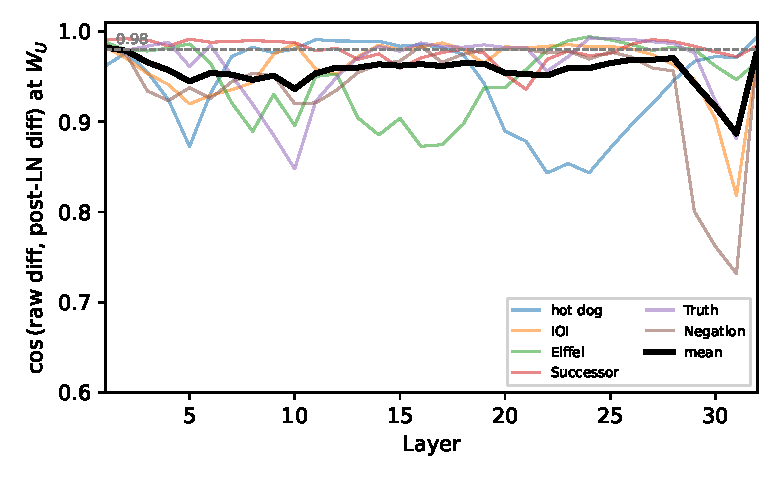
\includegraphics[width=0.62\textwidth]{ln_cosine.pdf}
\caption{Cosine between the raw ($\text{LN}_f$-bypassed) and strictly
normalized difference projections at $\WU$, per layer, for the six
poster cases (thin) and their mean (thick). L0 is omitted (the
read-position token is shared, so the differenced state is zero).}
\label{fig:ln}
\end{figure}

Raw and normalized projections diverge in \emph{magnitude}: residual-stream norms grow across
layers (from 4 at L1 to 175 at L31), so raw $\Delta$logits norms are not comparable
across layers. Where we report norms across layers (e.g., \S5.3), we use the
relative norm $\|\dhh\| / \|h_c\|$ to remove this scale artifact. Bypassing $\text{LN}_f$
means the projection relies on directional alignment between the residual
stream and $\WU$ rather than the calibrated magnitude that $\text{LN}_f$ would provide;
relative magnitude comparisons across layers should be interpreted
accordingly.

\paragraph{Why $\WU$, not $W_E$.} The input embedding matrix $W_E$ is an alternative
projection target --- fc1 reads from the residual stream, which originates as
$W_E$ embeddings. We test both. In Phi-2, the row vectors of $W_E$ and $\WU$ for identical
tokens are nearly orthogonal (mean cos 0.005 across the vocabulary). Projecting known clean MLP neurons' fc1
rows through $\WU$ produces interpretable labels (N925: ``food, food, foods'';
N7828: ``food, edible, delicious''; N841: ``husband, husbands, boyfriend'').
The same rows through $W_E$ produce noise (``union, replacement, abet'';
``required, when, executive''; ``Representative, postal, learning'').
Contrastive $\dhh$ shows the same pattern: $\WU$ reads ``tast, charred, crispy,
delicious'' for hot dog at L28; $W_E$ reads ``is, ern, erton.'' The alignment
gap widens with depth: fc1 rows' peak token-specificity via $\WU$ exceeds
$W_E$ by $1.02\times$ at L4, growing to $1.40\times$ at L28.

\subsection{Per-position reading}

By reading the contrast at every position, we trace information flow: at
which position does a meaning distinction first appear? Does it appear at
the differing token itself, or at a later position that attends to it?

\subsection{Attention and MLP decomposition}

Each transformer layer adds two components to the residual stream: attention
output and MLP output. We capture both via forward hooks and compute their
contrastive projections separately. This identifies which component writes a
given content distinction at each layer --- without causal intervention.

We note that a large contrastive norm in either component indicates that the
component's output differs between the two inputs, not that the component causes
the distinction. Causal verification (activation patching) is required to
establish causality.

\subsection{What the projection reads}

The contrastive projection re-ranks the logit lens through the input
design rather than through a learned decomposition. A raw logit-lens
readout of either input is dominated by signals the two inputs share
(often high-frequency function words at the top of the ranking); the
subtraction cancels the shared component and reads the remainder.

$\WU$ projection assigns token labels to directions in the residual
stream. At intermediate layers, these labels name the axis of variation
the contrast isolates: they localize where a distinction becomes legible
in token space. They do not certify its cause, and they are not an
account of everything the state carries; causal claims follow only from
the injection and patching tests below. The token labels are not
predictions of what the model will output at that layer.

\paragraph{Single-pair vs.\ multi-contrast readout.} A single contrastive pair
isolates one axis of variation, but the readout mixes the target signal
with content specific to that baseline. When the target concept
is a single entity (a name, a city), the pair-specific content is small
and the readout is clean. When the target is compositional (a food compound,
a moral judgment, a quantifier's pragmatic force), pair-specific content
can dominate the readout, producing
uninterpretable tokens. Each baseline contributes its own legitimate
signals --- ``fish'' adds fishing-related content, ``bus'' adds transportation
content --- alongside the shared illness signal. Multi-contrast
triangulation --- contrasting the same target against several baselines and
averaging --- cancels the signals that vary across baselines and preserves
the shared causal component.

We verify this empirically in \S3.3.

\paragraph{Read position and stability.} Contrastive reads taken at
the very start of a prompt are unstable: semantically irrelevant
changes, such as capitalising the first word, can shift the readout.
A shared preamble, identical across the pair and therefore cancelled
by the subtraction, moves the read into a stable region where the
target contrast dominates. We do not determine why the start is
unstable: it may reflect the attention-sink and massive-activation
structure present near the beginning of a sequence \citep{sun2026},
or the model still settling register and topic before the small target
difference can dominate. The examples in this paper use bare prompts
for clarity. For a well-separated lexical contrast the preamble is
only a refinement: the distinction survives without it (food
vocabulary dominates the late-layer readout either way) and merely the
specific tokens shift. It can, however, be essential: read at a
position where the two continuations are about to diverge, a bare
contrast can decode to register and next-token soup, while reading the
same pair inside a shared frame, a few tokens away from that
divergence, recovers a legible causal reading.

\section{Validation}

\subsection{The full activation delta is causal}

The probe is exploratory. As a baseline,
we test whether the full activation delta $\dhh[L] = h_\text{context}[L] - h_\text{control}[L]$
contains the causal information by injecting it into the control's residual
stream at layer $L$ and measuring prediction gap recovery. This is standard
activation patching: adding $\dhh$ to the control effectively replaces its
activation with the context's at that layer, so recovery at late layers is
expected. The interesting result is the \emph{layer profile} --- at which layer does
recovery onset, and does this match the contrastive readout?

\begin{table}[htbp]
\centering
\small
\begin{tabular}{lrrrrrrr}
\toprule
Case & L4 & L12 & L20 & L24 & L28 & L31 & Peak $z$ \\
\midrule
hot dog $\rightarrow$ delicious & 0\% & 5\% & 73\% & 80\% & 133\% & 150\% & 4249 \\
IOI $\rightarrow$ Mary & 0\% & 0\% & 0\% & 5\% & 75\% & 113\% & 525 \\
Eiffel $\rightarrow$ Paris & 0\% & 0\% & 2\% & 55\% & 73\% & 66\% & 1778 \\
Successor $\rightarrow$ Tuesday & 0\% & 0\% & 0\% & 11\% & 87\% & 98\% & 223 \\
\bottomrule
\end{tabular}
\caption{Prediction-gap recovery from injecting the full activation delta $\dhh[L]$ at one layer, for four cases (percent of the clean--control gap). Random directions of equal norm give zero mean recovery; the final column reports the $z$-score against that null.}
\label{tab:recovery}
\end{table}

Recovery is zero at early layers and clear by L28--31 (75--150\%).
Recovery above 100\% means that the injected $\dhh$ overshoots the
target prediction. This is expected: $\dhh$ captures the full
difference between the two residual streams, but the control's own
residual stream at late layers already encodes partial prediction
content, so adding the full difference on top of that partial encoding
exceeds the target.
Random directions of the same norm give zero mean recovery at every layer
($z = 223$--$4249$). This establishes that the \emph{direction} of $\dhh$ matters, not
just its norm --- but a random direction is a weak null: it is near-orthogonal
to every meaningful direction, so beating it is easy. The near-neighbour
control below is the sharper test, and Section 3.3 tests whether the
token-readable component of $\dhh$ carries the causal content.

\paragraph{Near-neighbour contrasts.} A sharper test replaces the random
direction with a \emph{same-frame near-neighbour} contrast of equal norm.
For the hot-dog case, we inject $\dhh$ from ``The X dog was'' minus ``The
cold dog was,'' norm-matched to the true contrast, for seven adjectives.
Non-food adjectives (warm, big, wet, angry) recover $\approx 0\%$ at every
layer. ``Delicious'' also recovers $\approx 0\%$ despite being a food word:
the compound recognition is specific to ``hot dog,'' not to any food
adjective before ``dog.'' ``Fried'' partially recovers (12--20\%,
$\cos = 0.81$ with the true direction at L28), consistent with ``fried
dog'' sharing part of the food-compound path. Recovery is specific to the
content of the contrast, not a generic effect of adding a same-norm
structured direction at that position.

\paragraph{Recovery onset.} Hot dog recovery begins at L12 (5\%),
rising sharply at L20 (73\%) --- the layers where food vocabulary appears in the
contrastive projection at the prediction position. IOI recovers from L24
(where ``Mary'' first dominates the readout). Factual recall recovers from L20
(where ``France'' first appears).

\subsection{Dose-response and bidirectional causality}

The layer-sweep above injects the full $\dhh$ at one layer. We can also extract a
specific contrastive \emph{direction} from multiple pairs and test its causal effect
with controlled magnitude.

\paragraph{Eatability direction.} We extract a food-compound direction by averaging the
contrastive (hot dog minus X dog) for X $\in$ \{cold, angry, old, pet, stray\} at
the dog position, L4 post. These five directions are mutually consistent
(pairwise cos 0.72--0.84). We inject the mean direction into non-food prompts
at the dog position at varying fractions of its natural magnitude. Note that
cold dog and angry dog are in the extraction set; the injection test measures
whether the averaged direction produces graded, dose-dependent effects on
model output, not whether it generalizes to held-out prompts. The
multi-contrast triangulation experiments (\S3.3, Table~\ref{tab:triangulation}) provide the held-out
generalization test, where the shared component is extracted from one set of
baselines and recovery is measured on a different baseline.

Greedy generation shows the induced shift is semantic, not a
single-token artifact:

\begin{table}[htbp]
\centering
\small
\begin{tabularx}{\textwidth}{llY}
\toprule
Prompt & Injection & Greedy continuation \\
\midrule
The cold dog was & baseline & shivering in the snow, so the owner put a sweater on it. \\
The cold dog was & $+0.50\times$ & more popular than the hot dog because the cold dog was easier to eat. \\
The cold dog was & $+1.00\times$ & more expensive than the hamburger because the hamburger was made with better quality ingredients. \\
The angry dog was & baseline & barking loudly at the mailman. \\
The angry dog was & $+1.00\times$ & more expensive than the hamburger because the hamburger was cheaper. \\
\bottomrule
\end{tabularx}
\caption{Greedy continuations under eatability injection, confirming a coherent semantic shift rather than a single-token artifact.}
\label{tab:eatability-greedy}
\end{table}

Subtracting the same direction from ``The hot dog was'' reverses the effect (Table~\ref{tab:eatability-reverse}):

\begin{table}[htbp]
\centering
\small
\begin{tabularx}{\textwidth}{llY}
\toprule
Prompt & Injection & Greedy continuation \\
\midrule
The hot dog was & baseline & too spicy for the child\ldots \\
The hot dog was & $-1.00\times$ & more popular than the cold dog because the hot dog was more appetizing. \\
The hot dog was & $-1.50\times$ & panting heavily, so the owner gave it some water to cool down. \\
\bottomrule
\end{tabularx}
\caption{Subtracting the eatability direction from ``The hot dog was'' reverses the effect (greedy continuations).}
\label{tab:eatability-reverse}
\end{table}

At $+1.0\times$, ``The cold dog was'' generates a food-comparison sentence. At $-1.5\times$,
``The hot dog was'' generates an animal-care sentence. The minimum dose that
flips top-1 prediction is $0.30\times$ for cold dog (where ``cold'' partially aligns
with food) and $0.65\times$ for angry dog (where ``angry'' strongly primes the animal
reading).

\paragraph{Truth direction.} We extract a truth/falsity direction by averaging the
contrastive (true statement minus false statement) for five fact pairs (Paris/France,
water/$100^\circ$, Sun/star, dogs/mammals, Tokyo/Japan) at the prediction
position. As with the eatability demonstration, the statements injected
below overlap the extraction set; the leave-one-out replication at the
end of this section provides the held-out test. Injecting into false
statements (Table~\ref{tab:truth-inject}):

\begin{table}[htbp]
\centering
\small
\begin{tabularx}{\textwidth}{llY}
\toprule
Prompt & Injection & Greedy continuation \\
\midrule
Paris is not the capital of France. This statement is & baseline & false. Paris is the capital of France. \\
Paris is not the capital of France. This statement is & $+0.50\times$ truth & true. \\
Paris is not the capital of France. This statement is & $+1.00\times$ truth & true. \\
Dogs are reptiles. This statement is & baseline & false. \\
Dogs are reptiles. This statement is & $+1.00\times$ truth & true. \\
\bottomrule
\end{tabularx}
\caption{Injecting the averaged truth direction into false statements flips the model's verdict (greedy continuations).}
\label{tab:truth-inject}
\end{table}

Subtracting from true statements (Table~\ref{tab:truth-subtract}):

\begin{table}[htbp]
\centering
\small
\begin{tabularx}{\textwidth}{llY}
\toprule
Prompt & Injection & Greedy continuation \\
\midrule
Paris is the capital of France. This statement is & baseline & true. \\
Paris is the capital of France. This statement is & $-1.0\times$ truth & false. Paris is the capital of France, but it is not the only city\ldots \\
The Sun is a star. This statement is & baseline & true because we know that the Sun is a star based on scientific evidence\ldots \\
The Sun is a star. This statement is & $-1.0\times$ truth & false. The Sun is a star, but it is not the only star in the universe\ldots \\
\bottomrule
\end{tabularx}
\caption{Subtracting the truth direction from true statements flips the verdict (greedy continuations).}
\label{tab:truth-subtract}
\end{table}

Scaling the extraction to 15 fact pairs and testing by leave-one-out
(the direction is averaged from the other 14 pairs and injected at the
final position of the held-out statement, extracted at L20) confirms
the effect on held-out statements: at twice the natural magnitude, all
15 false statements flip to ``true'' and all 15 true statements to
``false'' (10/15 and 7/15 at natural magnitude).

The truth direction has lower cross-pair consistency (mean pairwise
cos 0.36 across the 15 pairs) than the
eatability direction (0.72--0.84), reflecting the fact that ``what makes Paris-is-the-capital
true'' and ``what makes dogs-are-mammals true'' share less structure
than different food-compound contrasts. The lower consistency, and the
need for above-natural magnitude to flip every held-out statement,
suggest the truth direction is noisier than the lexical axes and may
benefit from the multi-contrast triangulation of \S3.3.

\subsection{Multi-contrast triangulation recovers compositional signals}

For compositional contrasts, single-pair readout may fail because the
target signal is mixed with pair-specific content. We test whether
multi-contrast triangulation recovers the causal component.

For ``She caught a cold'' vs ``She caught a fish,'' we project the single-pair
$\dhh$ onto the subspace spanned by the $\WU$ rows of its top-20 and bottom-20
tokens (40 directions total, orthogonalized via QR decomposition) and
inject only this token-subspace component. This recovers 1\% of the
prediction gap --- the token-readable part of the single-pair $\dhh$ is not
where the causal content lives. (By contrast, injecting the full
unrestricted $\dhh$ at the same layer recovers 69\% --- the causal content is
present but not aligned with the loudest $\WU$ directions.) The same case
triangulated against five baselines yields an averaged $\dhh$ whose
token-subspace component --- constructed the same way, from the $\WU$
rows of the averaged vector's own top-20 and bottom-20 tokens --- reads
``doctor, doctors, rest, see'' and recovers 77\%. The comparison is
therefore apples-to-apples: both numbers inject only the token-readable
component. The five baselines are:

\begin{itemize}[leftmargin=*]
\item ``She caught a \textbf{fish} and went to'' (physical catch)
\item ``She caught a \textbf{ball} and went to'' (physical catch)
\item ``She caught a \textbf{bus} and went to'' (transportation)
\item ``She caught a \textbf{thief} and went to'' (apprehension)
\item ``She caught a \textbf{glimpse} and went to'' (perception)
\end{itemize}

Each baseline shares the ``caught a \rule{1em}{0.4pt}'' frame but differs in what was caught.
The shared component across all five contrasts --- what ``cold'' has that fish,
ball, bus, thief, and glimpse do not --- is the illness signal. Multi-contrast
averaging isolates this from the pair-specific content (e.g., medical vs
fishing in the cold/fish pair alone) that dominates the single-pair readout
(Table~\ref{tab:triangulation}).

% KNOWN DEFECT (2026-07-30, do not re-publish without fixing): the
% "Multi-contrast recovery" numbers below (77/75/49/101) are rank-1
% shared-axis injections (deep_decompose.py rec_s), NOT the token-subspace
% construction 3.3 describes. Token-subspace triangulation recovers 7/4/7/-32
% at L28 (peaks 25-45% mid-late). Verified: triangulation_table_verify.py;
% session_report_2026-07-30_triangulation_table_verification.md. The
% "apples-to-apples" sentence above and the abstract's "1% -> 77%" inherit
% this. Plan: this paper is likely superseded by the bbxnlp version (which
% presents triangulation qualitatively and is unaffected); README carries
% the public note.
\begin{table}[htbp]
\centering
\small
\begin{tabular}{lrrl}
\toprule
Case & Single-pair recovery & Multi-contrast recovery & Shared component reads \\
\midrule
IOI (Mary/John) & 84\% & --- (not needed) & Mary, mary \\
Capital (Paris/Berlin) & 97\% & --- (not needed) & Paris, French \\
Caught a cold & 1\% & 77\% & doctor, doctors, rest \\
Theft/moral & 4\% & 75\% & evade, hoped, evasion \\
Hot dog food & 11\% & 49\% & crispy, charred, cooked \\
Some/all (partitive) & $-40$\% & 101\% & some, Some, SOME \\
\bottomrule
\end{tabular}
\caption{Single-pair $\WU$ projection vs.\ multi-contrast triangulation.
Entity-identity contrasts (top rows) read cleanly from a single pair. Compositional
contrasts (bottom rows) require multiple baselines to isolate the
token-shaped causal signal from pair-specific content.}
\label{tab:triangulation}
\end{table}

\paragraph{Why averaging works.} A companion paper derives the detection
arithmetic for this readout \citep{tuomi2026visibility}: a token-aligned
component carrying an energy fraction $f$ of the difference vector
surfaces in the top-$k$ only above a visibility threshold
$f^{*} \approx 2\ln(2V)/d$ (about 0.9\% of the vector's energy for
Phi-2), and averaging $N$ matched difference vectors suppresses the
incoherent remainder by $\sqrt{N}$, lowering the detection bar roughly
$N$-fold. The single-pair failures in Table~\ref{tab:triangulation} are
consistent with sub-threshold aligned energy rather than absent content;
averaging does not sharpen the signal, it suppresses the unaligned
remainder.

\paragraph{Granularity.} Multi-contrast averaging recovers what is shared across
baselines, but cannot determine whether the result is a single feature or
a stable bundle of co-occurring features. Entity-identity contrasts
(Mary/John) recover a component that corresponds to one token.
Compositional contrasts (illness, food-compound) may recover a bundle:
``doctor, rest, see'' could reflect co-activated medical, recovery, and
action features rather than a single ``illness'' feature. We do not claim
to recover atomic features. The method recovers the shared causal
component at the granularity the contrast design provides.

\subsection{Null model: smoothness is structural, not semantic}

$\WU$ contributes the interpretable token labels. Trajectory smoothness
(consecutive-layer cosine $\sim$0.9) is a general property of the residual stream,
not specific to meaningful contrasts: unrelated pairs (``The hot dog was'' vs
``Quantum mechanics is'') are equally smooth ($0.93 \pm 0.01$, $N=40$) as minimal
pairs ($0.88 \pm 0.03$, $N=6$), because any two residual streams diverge gradually.
Random directions give cosine $\sim$0.00 ($z = 64$--$93$), confirming $\dhh$ is structured
rather than noise, but smoothness alone does not validate content.

\subsection{Baseline subtraction}

A contrastive projection requires a second prompt. A generic
alternative is to subtract the mean residual of many random text
snippets of the same length (100 in our case), removing what is
common to arbitrary English text at this position and leaving
whatever is specific to the target. This achieves for a single prompt
what the paired subtraction achieves for a pair: the raw logit lens
is dominated by high-frequency function words (``a, the'') at every
layer, burying content tokens below them; after baseline subtraction,
the function words cancel and content surfaces.

Table~\ref{tab:decomposition} applies this to the hot-dog example
read inside a shared preamble (\S2.4). In the raw logit lens, food
tokens rank 300--1200 at intermediate layers, invisible below function
words. After baseline subtraction they surface to the top.

\begin{table}[htbp]
\centering
\small
\begin{tabular}{@{}r@{\;\;}l@{\;\;}l@{}}
\toprule
\textbf{L} & \textbf{Raw logit lens} & \textbf{Baseline-subtracted} \\
\midrule
6  & not, only, always            & eaten\,\textsuperscript{+2}, foods, menu \\
10 & not, indeed, always          & flavor\,\textsuperscript{+3}, sold, cheese \\
16 & not, only, always            & cheese\,\textsuperscript{+4} \\
20 & not, more, only              & delicious\,\textsuperscript{+8}, cheese, flavors \\
24 & not, more, a                 & cooked\,\textsuperscript{+19}, grilled, delicious \\
28 & not, a, the                  & cooked\,\textsuperscript{+30}, grilled\,\textsuperscript{+29}, sausage \\
\bottomrule
\end{tabular}
\caption{Raw logit-lens top tokens vs.\ baseline-subtracted top tokens
(Phi-2, final position). The raw projection reads ``not, only, always''
at every layer (function words dominate). After subtracting the mean of
100 random text snippets, food vocabulary surfaces from L6 onward and
builds through L28 --- content that ranks 300--1200 in the raw projection.}
\label{tab:decomposition}
\end{table}

\section{Lexical disambiguation}

\subsection{Compound noun: hot dog}

\textbf{Prompts:}
\begin{itemize}[leftmargin=*]
\item ``The hot dog was'' (food item)
\item ``The cold dog was'' (cold animal)
\end{itemize}

\textbf{Predictions:} hot dog $\rightarrow$ ``too'' (0.088), ``more'' (0.080), ``cooked'' (0.063);
cold dog $\rightarrow$ ``sh[ivering]'' (0.447), ``shaking'' (0.036).

\textbf{Per-position trace (4 tokens: The, hot/cold, dog, was):}

At position 2 (``dog'') --- same token in both prompts, L0 contrast is zero:
\begin{itemize}[leftmargin=*]
\item L1: ``hot, molten, fiery'' --- ``dog'' receives temperature info from ``hot''
\item L4 (post-MLP): ``fried'' first appears --- compound meaning recognized by MLP
\item L5 (post-attention): ``fried'' persists --- L5 attention adds little locally
\item L24: ``fried, seasoning, Flav, Serv, vendor'' --- full food vocabulary
\item L32: ``vendor, vendors, stand, topping'' --- hot dog stand
\end{itemize}

Sub-layer decomposition at L4--L5 confirms the compound is recognized by the
MLP at L4, not by attention. The MLP contrastive norm at L4 (20.0) dominates
the attention norm (3.8); ``fried'' appears in the MLP output but not the
attention output. L5 attention writes orthogonally to the food direction
($\cos(\Delta\text{pre}, \Delta\text{attn}) < 0.08$ across all contrasts tested).

At position 3 (``was'') --- reads from ``dog'':
\begin{itemize}[leftmargin=*]
\item L5 (attention): ``delicious, substitutes, cooked'' --- food signal arrives via
  attention from ``dog'' (one layer after MLP recognizes the compound at ``dog'')
\item L6: ``fried, delicious, tasty, breakfast''
\item L28: ``tasty, charred, crispy, delicious, spicy'' (hot) vs ``grooming, shudder, shaking'' (cold)
\end{itemize}

\textbf{Attention routing at L5, position ``was'':}
Head 19 attends to ``dog'' position with weight 0.911 in the hot-dog context vs
0.735 in cold-dog. Head 29 attends 0.345 vs 0.138. These heads read the
compound-noun information from ``dog'' and write it to ``was.''

\textbf{Multi-contrast convergence:} The food-compound direction is stable across
reference points. Five different contrasts (hot dog minus cold/angry/old/pet/stray
dog) produce pairwise cosine 0.72--0.84 at the dog position, confirming
the signal is about food-compound identity, not temperature or emotion. Note
that high pairwise cosine between full $\dhh$ vectors does not imply high
recovery from their top $\WU$ token directions (Table~\ref{tab:triangulation} reports 11\% for hot
dog). The cosine measures alignment of the full d-model vectors; the 11\%
measures how much of each vector lives in the subspace of its loudest $\WU$
tokens. A signal can be consistent in direction (high cosine) while being
distributed across many $\WU$ directions rather than concentrated in a few
(low token-subspace recovery).

\textbf{Neuron and head detail:} The MLP write at ``dog'' is
distributed: the ten neurons pushing hardest along the food direction
carry only $\sim$10\% of it, spread across hundreds, some writing food
(one writes ``cooked, foods, dishes'') and some suppressing animal
content (another writes ``dogs, puppies''). The routing head L5.H19,
already flagged above by its attention to ``dog,'' writes ``cooked,
eaten'' into ``was'': the edibility signal the read surfaces at the
prediction position. The readable food content is thus genuinely
computed, but by a distributed MLP write plus a localized routing head,
not by any single neuron.

\textbf{Activation patching at multiple layers and positions} (Table~\ref{tab:hotdog-patch}):

\begin{table}[htbp]
\centering
\small
\begin{tabular}{lllll}
\toprule
Position patched & Layer & P(food) & Top-1 & Effect \\
\midrule
(baseline hot dog) & --- & 0.142 & ``too'' & --- \\
dog (pos 2) & L0--L4 & 0.000 & ``pant'' & Food eliminated \\
dog (pos 2) & L5 & 0.094 & ``more'' & Food partially survives \\
dog (pos 2) & L12+ & 0.12--0.14 & ``too'' & Near baseline \\
hot (pos 1) & L0--L28 & 0.11--0.14 & ``too'' & Minimal effect at all layers \\
was (pos 3) & L0--L5 & 0.13--0.14 & ``more'' & Food preserved \\
was (pos 3) & L12 & 0.058 & ``placed'' & Food declining \\
was (pos 3) & L20+ & 0.005 & ``sh'' & Food eliminated \\
\bottomrule
\end{tabular}
\caption{Activation patching of the hot-dog prompt at three positions and several layers, tracing the two-hop MLP$\rightarrow$attention chain (P(food) and top-1 token).}
\label{tab:hotdog-patch}
\end{table}

The patching traces the two-hop chain precisely. (1) Patching ``dog'' at L0--L4
eliminates the food signal entirely --- the compound meaning has not yet been
computed. At L5, just after the L4 MLP write where ``fried'' first
appears in the contrastive projection, food partially survives the
patch --- the computation is completing at these layers. By L12+ the patch has minimal effect. (2) Patching ``hot'' has no effect
at any layer --- its information has already been copied to ``dog'' via L0
attention. (3) Patching ``was'' has no effect at L0--L5 (the food information
hasn't arrived yet) but eliminates food from L12 onward --- consistent with
attention at L5--6 copying the compound meaning from ``dog'' to ``was.''

\textbf{Mechanism:} Attention at L0 copies ``hot'' to the ``dog'' position. The MLP at
L4 recognizes the compound at the ``dog'' position (``fried'' first appears in the
MLP output). Attention at L5 broadcasts this from ``dog'' to ``was'' (H19,
attn=0.91). The contrastive projection identified each of these stages; activation
patching at three positions and multiple layers confirms the information flow.

\subsection{Other disambiguation cases}

The same method traces disambiguation in verb-object pairs and noun ambiguity:

\textbf{``He caught a cold and'' vs ``He caught a fish and''} (verb meaning changes):
\begin{itemize}[leftmargin=*]
\item L12: ``contracted, virus, contagious'' (cold pole)
\item L28: ``fever, coughing, cough, flu'' vs ``proudly, reel, bait, trout''
\end{itemize}

\textbf{``The bank was steep and'' vs ``The bank was closed and''} (noun disambiguated by
adjective):
\begin{itemize}[leftmargin=*]
\item L12: ``climb, inclined, steep'' (terrain pole)
\item L27--28: ``bank, banks, banking'' reappear in the contrastive projection ---
  the noun's representation is revisited after the modifier has disambiguated
  it. This is compatible with a two-pass pattern (resolve meaning from the
  modifier, then update the noun representation), though the contrastive
  projection reads content, not mechanism.
\end{itemize}

\textbf{``He was fired up and'' vs ``He was fired and''} (particle changes meaning):
\begin{itemize}[leftmargin=*]
\item L28: ``excited, ready, energetic'' (fired up) vs ``sued, blacklist, lawsuits''
  (fired)
\end{itemize}

\subsection{Scalar implicature: pragmatic inference in the residual stream}

Lexical disambiguation (\S4.1--4.2) traces how the model resolves word meaning.
A different kind of distinction involves quantifiers: ``Some of the students
passed'' and ``All of the students passed'' produce different continuations.
We trace how the residual stream diverges between these two quantifiers.

\textbf{Design:} Contrast ``Some of the students passed the exam, so'' against
``All of the students passed the exam, so'' and read the contrastive projection
at the final token.

\textbf{Trajectory (some pole $+$, all pole $-$)} (Table~\ref{tab:somall-traj}):

\begin{table}[htbp]
\centering
\small
\begin{tabular}{lll}
\toprule
Layer & Some pole reads & All pole reads \\
\midrule
L8 & might, may & except, together \\
L20 & Others, another & everyone, except, Everyone \\
L28 & others, Others, another & everyone, Everyone, everybody, except \\
\bottomrule
\end{tabular}
\caption{Contrastive trajectory for the some/all quantifier contrast (positive pole = some, negative pole = all).}
\label{tab:somall-traj}
\end{table}

The negative pole consistently reads ``everyone, everybody, except'' from L8
onward --- tokens associated with ``all'' contexts. This reflects the divergent
prediction trajectories of the two quantifiers: the ``all'' context primes
totality tokens, and the contrastive projection surfaces this divergence.
Whether this reflects an internal ``not everyone'' computation or simply the
output distribution difference between the two prompts cannot be determined
from the contrastive readout alone.

\textbf{Cross-content consistency.} The same some/all contrast across 6 noun
phrases (students, cookies, houses, employees, books, countries) produces
pairwise cosine 0.12--0.45 (mean 0.30). The negative pole consistently reads
totality words (``everyone, all, except, none'') across all noun phrases,
while the positive pole varies with content. Using multi-contrast
triangulation across noun phrases, the shared component reads ``Others,
Other, another'' vs ``all, everyone, none, except, everybody'' --- both poles
token-shaped.

\textbf{Scalar gradient.} Projecting five quantifiers (None, Few, Some, Most,
All) onto the some$\leftrightarrow$all axis at L28 (Table~\ref{tab:scalar-gradient}):

\begin{table}[htbp]
\centering
\small
\begin{tabular}{lr}
\toprule
Quantifier & Projection \\
\midrule
None & $+27$ \\
Few & $+14$ \\
Some & $+84$ \\
Most & $+13$ \\
All & 0 (baseline) \\
\bottomrule
\end{tabular}
\caption{Projection of five quantifiers onto the some$\leftrightarrow$all axis at L28. ``Some'' is the outlier, consistent with its status as the pragmatically marked quantifier.}
\label{tab:scalar-gradient}
\end{table}

The gradient is not monotonic: ``Some'' is the outlier, projecting far beyond
any other quantifier. ``Few'' and ``Most'' project similarly despite being
semantically opposite. This is consistent with ``some'' being the
pragmatically marked quantifier --- the one that generates scalar implicature
--- rather than the scale reflecting quantity.

\textbf{Explicit vs bare.} Contrasting ``Some of the students passed'' against
``Some but not all of the students passed'' produces a non-trivial $\dhh$ (norm
57--59 at L28). The $-$side reads ``some, Some, not, neither, but, BUT'' --- the
explicit restriction changes the representation. The bare ``some'' computes
partial implicature (the ``everyone/except'' signal), but adding ``but not all''
adds further restriction beyond what the bare form computes.

\section{Replicating landmark findings}

\subsection{Indirect object identification}

The IOI circuit~\citep{wang2023} identifies how GPT-2 resolves which name a
pronoun refers to. We replicate the core finding with the contrastive method.

\textbf{Design:} Contrast ``John and Mary went to the store. John gave a book to'' vs
the same with names swapped. The IO name should appear in the contrastive
projection at the prediction site.

\textbf{Prompts (example):}
\begin{itemize}[leftmargin=*]
\item A: ``John and Mary went to the store. John gave a book to'' $\rightarrow$ Mary
\item B: ``Mary and John went to the store. Mary gave a book to'' $\rightarrow$ John
\end{itemize}

\textbf{Contrastive trajectory:}
\begin{itemize}[leftmargin=*]
\item L8: gender emerges (``himself, his'' vs ``herself, her'')
\item L24: IO names appear (``Mary, Mary'' vs ``John, John'')
\item L28: fully stable (``Mary, Mary, mary'' vs ``John, John, john'')
\end{itemize}

\textbf{Per-head decomposition at L24:} Decomposing the attention output by head
identifies which heads carry the IO name. Three heads dominate consistently
across three name pairs (John/Mary, Alice/Bob, Dan/Eve; Table~\ref{tab:ioi-heads}):

\begin{table}[htbp]
\centering
\small
\begin{tabular}{lrrrl}
\toprule
Head & John/Mary (norm) & Alice/Bob & Dan/Eve & Content \\
\midrule
H14 & 8.3 & --- & 11.4 & IO name (MD/Mary, de/draw) \\
H1 & 7.5 & 5.9 & 7.0 & IO name (Mary, Bob, ever/ves) \\
H16 & 3.4 & 4.5 & 12.8 & IO name (Mary, Bob, Eve) \\
\bottomrule
\end{tabular}
\caption{Per-head contrastive norm at L24 for the IOI name-swap contrast across three name pairs. Three heads carry the indirect-object name.}
\label{tab:ioi-heads}
\end{table}

These heads have the largest contrastive norms at L24 and read IO-name tokens
when projected through $\WU$. No other head exceeds norm 3.0 consistently. This
identifies heads that carry the IO name signal --- the same observational
signature as the name-mover heads that~\citet{wang2023} found in GPT-2, here
located in Phi-2 using only contrastive projection.

\textbf{Why the name-swap contrast cannot test routing.} Prompts A and B run the
identical IOI algorithm --- detect the duplicated subject, suppress it, copy the
other name --- and differ only in which tokens fill the roles. The shared
algorithm cancels under subtraction, so the heads the contrast surfaces are
name-content carriers, not the routing mechanism. Three tests sharpen what they
are and whether they are causal.

\textbf{Attention patterns confirm two genuine name-movers.} At L24, H14 and H16
attend from the final position to the IO token (``Mary''), with 0.86 and 0.56 of
their attention mass on it --- reading the indirect object directly, the
name-mover signature. H1, also flagged by contrastive norm, instead attends to
the sequence-initial sink token (0.87): it is a false positive of the norm
criterion that the attention pattern filters out. Pairing contrastive norm with
attention direction separates the readers (H14, H16) from sink heads.

\textbf{Ablation and denoising agree: the heads are not the causal carrier.}
Ablating all three heads at L24 (zeroing their pre-projection output at the last
position) reduces P(Mary) from 0.696 to 0.685 --- a 1.1\% drop; individual
ablation gives H14 $-0.2$\%, H16 $-0.9$\%, H1 none. Three control heads (H0, H5, H10)
give a comparable 0.3\% drop and the generation is unchanged. Denoising is the
more sensitive complement: we corrupt the prompt by swapping the giver
(P(Mary) = 0.011) and patch clean head outputs back at the final position,
measuring how much of the clean--corrupt gap (toward 0.696) is restored.
Patching the name-movers restores $\le$1\%; patching all 32 heads at the final
position restores $\le$2\% --- at every layer from L20 to L28. Injection gives the
same verdict for sufficiency: the name-movers' contrastive output (A$-$B)
shifts P(Mary) in B from 0.026 to only 0.037 at $1\times$ and 0.067 at $3\times$, and
patching all 32 heads A$\rightarrow$B reaches only 0.041. By contrast, injecting the full
residual-stream $\dhh$ at L28 drives P(Mary) to 0.642. The decision is carried by
the cumulative residual stream, not by any layer's attention write at the
final position.

\textbf{A structure-preserving contrast surfaces a name-invariant signal.} Contrasting
the IOI prompt against a no-duplicate baseline (giver = a third name, ``Sam'')
keeps the duplicate-detection computation in the subtraction. This surfaces
different heads --- at L26 one reads the giver name (``Sam''), others read
structural tokens --- and the resulting delta does not project to clean tokens
through $\WU$.

$\WU$-illegibility alone is weak evidence for structure, however: a
token-aligned component can be present yet sit below the readout's
detection threshold \citep{tuomi2026visibility}. We test the claim
directly with prompt design rather than a trained probe. Build a family of eight name-sets that share the IOI structure
but vary the token identities (John/Mary, Alice/Bob, \ldots), and form both contrasts
at END for each set. As depth increases the two diverge sharply: the name-swap
(token) direction rotates with the names and collapses toward orthogonality
across the family (mean pairwise cosine $+0.73$ at L20 $\rightarrow$ $+0.21$ at L24 $\rightarrow$ $+0.01$ at
L28), whereas the no-duplicate direction stays aligned ($+0.83$ $\rightarrow$ $+0.66$ $\rightarrow$ $+0.37$).
Averaging each contrast over the family --- which cancels token-specific
components and keeps the shared one --- preserves 0.83 of the no-duplicate norm at
L24 against 0.56 for the name-swap. The averaged name-swap survivor reads as
$\WU$ junk (its per-set reads are clean but different names --- ``Mary'', ``Sam'' --- that
cancel), while the averaged no-duplicate survivor reads as identity-free
recipient-role content (``charity, share, shop, others''). Position-resolved
attention agrees: heads H12 and H20 read END$\rightarrow$duplicate-position across all eight
name-sets (0.16--0.37), keying on the \emph{position} regardless of which name fills
it --- a structural signature that never touches $\WU$.

The signal is therefore present, contrast-isolable, and name-invariant
where the name-identity content is not. (The
surviving direction reads as the recipient role, which is broader than
``inhibition'' specifically; separating routing from recipient-role content would
need a further control.)

\textbf{Tracing the path by position-resolved patching.} The corrupted (swapped)
prompt differs from the clean one in a \emph{single} input token --- the second
subject at position 9 (S2) --- so all causal divergence originates there. Patching
the full residual stream at one position from clean into the corrupted run,
across layers, traces where the information lives (recovery of P(Mary), corrupt
0.011 $\rightarrow$ clean 0.696):

\begin{table}[htbp]
\centering
\small
\begin{tabular}{lrrrrrrr}
\toprule
Patched position & L0 & L8 & L12 & L16 & L20 & L24 & L28 \\
\midrule
IO (pos 3) & 0\% & 0\% & 0\% & 1\% & 0\% & 0\% & 0\% \\
S2 (pos 9) & 100\% & 90\% & 79\% & 59\% & 16\% & 6\% & 0\% \\
END & 0\% & 0\% & 0\% & 1\% & 37\% & 59\% & 98\% \\
S2 + END & 101\% & 95\% & 88\% & 87\% & 96\% & 97\% & 100\% \\
\bottomrule
\end{tabular}
\caption{Position-resolved patching of the IOI prompt (recovery of P(Mary), corrupt $\rightarrow$ clean). The causal signal transfers from S2 to END between L16 and L28.}
\label{tab:ioi-path}
\end{table}

The IO position never matters --- its token is identical in both prompts. The S2
position carries all of the recovery at L0 and loses it monotonically, while END
gains it in lockstep; S2 and END jointly recover $\sim$100\% at every layer. The
causal signal transfers from S2 to END between L16 and L28, with the crossover
(END-only overtaking S2-only) at L18--20.

Attention identifies the heads that perform the transfer. At L18--20, heads
attending from END to S2 dominate (H10, H12, H20, H31) --- they move the
duplicate-subject signal forward. At L22--26, heads attending to the IO token
take over (H3, H14, H16, H0) --- the name-movers that read and write the indirect
object. This is the S-inhibition $\rightarrow$ name-mover structure of the IOI circuit,
spread across roughly eight heads and eight layers rather than concentrated in a
few.

This also resolves the apparent null of the per-head tests. The END residual
after L22 recovers 59--98\% of the prediction, but no single head's END output
does ($\le$2\%): the signal arrives via the cumulative S2$\rightarrow$END transfer, carried in
the residual stream, so ablating or patching any one head leaves the others to
reconstruct it.

\textbf{Summary.} Contrastive projection, with attention confirmation, correctly
identifies the genuine name-mover heads (H14, H16) and their read site (the IO
token), and exposes H1 as a sink-head artifact of the norm criterion.
Position-resolved patching then traces the full path: an identifiable origin
(S2), a transfer window (L18--22), and two head populations (S2-readers then
name-movers). The IOI computation in Phi-2 is distributed but fully traceable ---
no single head is necessary (ablation) or sufficient (per-head patching),
because the decision rides the cumulative residual stream. This differs from
GPT-2, where~\citet{wang2023} found the circuit concentrated in a few heads; here the
same algorithm is spread across many heads and layers, and the contrastive
method plus position-resolved patching recovers its structure end to end.

\textbf{Accuracy:} 160/160 on Phi-2 (40 name pairs $\times$ 4 templates; mean
IO$-$S logit margin 6.4, always positive), 30/30 on Pythia-1.4B (100\%),
29/30 on Pythia-410M (97\%).

\subsection{Factual recall}

\textbf{Design:} Contrast prompts requiring different factual answers.

\textbf{``The Eiffel Tower is located in'' vs ``The Colosseum is located in'':}
\begin{itemize}[leftmargin=*]
\item L20: ``French, France'' vs ``ancient, Roman, Alexandria''
\item L28: ``French, Paris'' vs ``Rome, Roma, Gladiator''
\end{itemize}

\textbf{Per-head decomposition:} At L24, H13 carries the largest contrastive norm
(3.9, reads ``France, French, Paris''). At L28, the signal distributes across
multiple heads (H21, H7, H0), consistent with the factual content spreading
from a concentrated source to a broader representation.

\textbf{Causal path trace.} To test whether this concentration is causal rather than
correlational, we use a single-token contrast --- ``The capital of \textbf{France} is''
($\rightarrow$ Paris) vs ``The capital of \textbf{Japan} is'' ($\rightarrow$ Tokyo) --- which differ in exactly
one input token, the subject. All causal divergence therefore originates at the
subject position, so position-resolved patching (restore the clean residual
stream at a chosen position and layer into the corrupt run; measure recovery of
P(Paris)) traces where the answer is built and when it moves. CLEAN P(Paris) =
0.806, CORRUPT = 0.001.

\begin{table}[htbp]
\centering
\small
\begin{tabular}{rrrr}
\toprule
layer & patch SUBJ only & patch END only & SUBJ+END \\
\midrule
L0--L16 & $\sim$100\% & $\sim$0\% & $\sim$100\% \\
L18 & 99\% & 10\% & 100\% \\
L20 & 74\% & 42\% & 100\% \\
L22 & 50\% & 57\% & 100\% \\
L24 & 8\% & 89\% & 100\% \\
L28 & 0\% & 99\% & 100\% \\
\bottomrule
\end{tabular}
\caption{Position-resolved patching for factual recall (recovery of P(Paris)). The answer is held at the subject token through the early layers, then handed to END around L22.}
\label{tab:fact-path}
\end{table}

The answer lives entirely at the subject position through L16--L18 (a flat
plateau: patching the subject alone fully restores Paris), then drains to the
END position over L18--L28, with the handoff crossover at \textbf{L22}. Patching
subject and END jointly recovers $\sim$100\% at every layer --- the signal rides the
cumulative residual along a single subject$\rightarrow$END path, with no third site. The
plateau-then-move shape matches the subject-MLP enrichment~\citet{meng2022}
and~\citet{geva2023} report for factual recall, and the handoff sits a few
layers later than IOI's (L22 vs L18--20).

Position-resolved attention from END names the carriers: attention to the
subject peaks at L24, with H16 (0.45) and \textbf{H13} (0.31) at the top ---
and H13 is the same
head the contrastive-norm decomposition independently flagged as reading
``France/French/Paris.'' The norm criterion (``this head's output differs'') and the
causal trace (``this head moves the subject signal to END'') converge on the same
unit.

\textbf{Generality.} The subject$\rightarrow$END structure replicates across 20
country/capital pairs: clean P(capital) averages 0.88 (all $\ge$ 0.5),
corrupt P $\approx$ 0, and the subject$\rightarrow$END crossover falls at
L22--L24 for every pair (median L24).

\textbf{Different factual domains:} ``The capital of France is'' vs ``The capital of
Japan is'' --- the contrastive reads ``Paris, France, French'' on the France pole
and ``Japanese, Japan, Tokyo'' on the Japan pole. Each entity's associated
knowledge cluster appears on its respective side.

\subsection{Factual recall vs hallucination}

When the model hallucinates --- producing a confident but fabricated answer for
a fictional entity --- the contrastive projection shows what the model's
retrieval surfaces in token space: specific facts for real entities, and
nothing beyond name fragments for fictional ones.

\textbf{Design:} We construct matched pairs where one prompt elicits genuine recall
and the other elicits hallucination, keeping the frame identical (Table~\ref{tab:halluc-prompts}):

\begin{table}[htbp]
\centering
\small
\begin{tabularx}{\textwidth}{YlYl}
\toprule
Real prompt & Prediction & Fictional prompt & Prediction \\
\midrule
Nikola Tesla, born in 1856, invented the & Tesla coil\ldots & Ludvig von Vogelkirche, born in 1859, invented the & first practical electric motor\ldots \\
Marie Curie, born in 1867, discovered & the elements polonium and radium\ldots & Helena Brandström, born in 1871, discovered & a new species of moth\ldots \\
\bottomrule
\end{tabularx}
\caption{Matched real/fictional entity prompts; both elicit confident, specific predictions.}
\label{tab:halluc-prompts}
\end{table}

Both sides produce confident, specific answers. But the contrastive projection
at L28 reads different content on each pole (Table~\ref{tab:halluc-poles}):

\begin{table}[htbp]
\centering
\small
\begin{tabular}{lll}
\toprule
Pair & Real pole (L28) & Fictional pole (L28) \\
\midrule
Tesla vs Vogelkirche & Tesla, alternating, Altern, electric & Vog, v, von, Von \\
Curie vs Brandström & radio, Radio, Radiation, radioactive & Brand, M, H, a \\
\bottomrule
\end{tabular}
\caption{Contrastive projection at L28: the real pole reads factual associations, the fictional pole only name fragments.}
\label{tab:halluc-poles}
\end{table}

The real pole reads \emph{factual associations} (Tesla $\rightarrow$ alternating current,
Curie $\rightarrow$ radioactivity). The fictional pole reads \emph{name fragments} (Vog, von,
Brand): the readout contains nothing about the entity beyond the tokens
of its name and their cultural associations.

\textbf{Confirmation via entity-vs-generic contrast.} Contrasting each entity
against a bare frame (``A person, born in 1856, invented the'') isolates what
the entity name adds. Tesla minus generic reads ``Tesla, alternating, AC'' at
L28 --- specific factual content. Vogelkirche minus generic reads ``Vog, von,
Von'' --- only name tokens. The readout for the hallucinated entity contains
no factual content beyond the name itself.

\textbf{Contrastive norm.} The relative norm $\|\dhh\|/\|h\|$ at L28 is systematically
larger for real-vs-fictional pairs (mean 0.98) than real-vs-real pairs (mean
0.70). Two real entities both occupy a shared subspace of factual-entity
representations, constraining their difference; a fictional entity lacks
factual content and drifts outside this subspace, producing a larger
contrastive norm against any real entity.

\textbf{Entropy.} The real inventors predict with lower entropy
(H = 1.5--2.5) than their fictional counterparts (H = 3.4--6.3),
consistent with the model having specific
knowledge to draw on. But entropy alone cannot distinguish ``confident recall''
from ``confident hallucination'' --- the mountain case illustrates this: Mount
Silverhorn (fictional) predicts ``2,856 meters'' at H = 2.8, within
reach of Mount Everest's H = 1.5. The contrastive projection shows the difference:
Everest's pole reads ``Nepal, Tibet, Himal'' (geographic knowledge), while
Silverhorn's reads ``1300, 1100, 1200'' (number-range priors calibrated to
``Southern Alps,'' not specific factual recall).

The contrastive projection does not find a ``hallucination flag.'' It reads
what the model's retrieval surfaces in token space, and for hallucinated
entities that readout contains only name tokens and contextual priors.
A caveat applies to every absence reading: a token missing from the
top-$k$ carries less aligned energy than the readout's visibility
threshold, which bounds the signal but is not evidence of zero signal
\citep{tuomi2026visibility}. What distinguishes the fictional entities
is that no factual content surfaces at any layer, where for the matched
real entities it does.

\subsection{Successor heads and temporal structure}

All successors are predicted correctly, including wrap-arounds:
``After Saturday comes'' $\rightarrow$ Sunday; ``After Sunday comes'' $\rightarrow$ Monday;
``After December comes'' $\rightarrow$ January.

\textbf{Contrastive trajectory:} Contrasting consecutive successors (e.g., ``After
Monday comes'' vs ``After Tuesday comes''), the contrastive projection at L24
reads the input day name on its respective pole (``Monday'' tokens positive,
``Tuesday'' negative). By L28 the successor day appears: ``Tuesday'' on the
Monday pole, ``Wednesday'' on the Tuesday pole. The successor computation is
visible as the transition from input-day to output-day content across layers.

\textbf{Per-head decomposition at L28:} Decomposing the contrastive signal by
attention head identifies H11 as the dominant successor head. Its contrastive
norm spikes at the Saturday$\rightarrow$Sunday and Sunday$\rightarrow$Monday transitions (Table~\ref{tab:successor}):

\begin{table}[htbp]
\centering
\small
\begin{tabular}{lrl}
\toprule
Day pair & H11 norm & Next-largest head \\
\midrule
Mon$\rightarrow$Tue & 2 & H20 (3) \\
Tue$\rightarrow$Wed & 3 & H20 (3) \\
Wed$\rightarrow$Thu & 3 & H20 (2) \\
Thu$\rightarrow$Fri & 4 & H20 (5) \\
Fri$\rightarrow$Sat & 4 & H25 (3) \\
\textbf{Sat$\rightarrow$Sun} & \textbf{11} & H12 (4) \\
\textbf{Sun$\rightarrow$Mon} & \textbf{11} & H12 (5) \\
\bottomrule
\end{tabular}
\caption{Per-head contrastive norm at L28 for consecutive-day successor contrasts. H11 dominates and spikes at the two week-boundary transitions.}
\label{tab:successor}
\end{table}

H11's norm triples at these two transitions; we do not have evidence for what
distinguishes them from the weekday transitions. The same head dominates
month-pair contrasts at L28, with norms 3--9 across all twelve transitions.

H11 dominates the successor signal but does not carry it alone --- H20 and H25
contribute at comparable norms for some day pairs (e.g., H20 norm=5 at
Thu$\rightarrow$Fri vs H11 norm=4).

A separate PCA analysis of the raw hidden states (not using the contrastive
projection) finds circular geometry for months and days; this is reported in
the supplementary materials as it does not use the paper's method.

\subsection{Parametric recall resists counterfactual assertion}

When in-context information contradicts parametric knowledge, does the model
override its stored facts? We test this by asserting a counterfactual capital
and then querying: ``The capital of France is Rome. The capital of France is.''

\textbf{The model does not override.} Across four country/capital pairs (France/Rome,
Japan/London, Germany/Madrid, Italy/Vienna), the model predicts the correct
parametric answer with high confidence despite the counterfactual assertion
(P(Paris) = 0.77 vs 0.81 baseline; P(Tokyo) = 0.87 vs 0.30 baseline). Even
with stronger framing (``It is well established that the capital of France is
Rome''), the model predicts Paris at 0.46. Only fictional framing (``In the
wizarding world'') partially weakens parametric recall (Paris 0.31, Rome 0.18).

\textbf{The contrastive trajectory reads correction, not acceptance.} Contrasting
the counterfactual assertion against the veridical one (Table~\ref{tab:counterfactual}):

\begin{table}[htbp]
\centering
\small
\begin{tabular}{lll}
\toprule
Layer & Counterfactual pole reads & Parametric pole reads \\
\midrule
L8 & similarly, similar & [subword fragments] \\
L20 & Actually, actually, actual & [subword fragments] \\
L24 & actually, Actually, correct & centrally, other \\
L28 & Actually, Greece, Paris & [comparison tokens] \\
\bottomrule
\end{tabular}
\caption{Contrastive trajectory contrasting a counterfactual capital assertion against the veridical one. From L20 the dominant signal is correction (``Actually'').}
\label{tab:counterfactual}
\end{table}

From L20 onward, the dominant signal is ``Actually, actually, correct'' --- the
model prepares a correction rather than accepting the override. At L28, the
Paris token logit is \emph{higher} on the counterfactual side ($+9.6$) than on the
veridical side --- the model strengthens its parametric recall when presented
with a contradicting assertion. The same holds for all four
country pairs.

\textbf{Distance weakens correction.} Inserting distractor text between the
assertion and query partially weakens the correction reflex: with a medium
distractor ($\sim$20 words), P(Paris) drops to 0.38 and P(Rome) rises to 0.16.
The contrastive trajectory at L28 shifts from reading ``Actually'' to reading
the asserted city (``Rome, Italy, Madrid''), suggesting the correction signal
decays with distance while the asserted content persists.

\textbf{Connection to hallucination (\S5.3).} The correction response --- ``Actually,
it is Paris'' --- requires the model to have retrieved the parametric fact.
The hallucination cases in \S5.3 show that fictional entities produce no
factual associations in the contrastive projection. The correction circuit
and the factual-retrieval circuit may share structure: both require that the
model has specific knowledge to draw on, and both are visible in the
contrastive trajectory as the presence or absence of factual content at
mid-to-late layers.

\section{Contrastive axis taxonomy}

Using 2$\times$2 factorial designs (crossing two binary axes, e.g., past/future $\times$
happy/sad), we measure whether each axis produces a consistent contrastive
direction across content. Consistency is the cosine between the axis direction
extracted from two different content fillers. We test 15 axes across four models
(Pythia-410M, Pythia-1.4B, Phi-2, Phi-4).

\subsection{Three tiers of axis consistency}

Axes partition into three tiers:

\textbf{Tier 1: Cross-family, token-readable} (cos $>$ 0.7 in all four models).
Eight axes exceed 0.7 consistency in all four models, though some weaken at
scale: code/natural language (0.88--0.95), positive/negated (0.84--0.90),
past/future (0.81--0.89), English/French (0.83--0.98, declines at scale),
assignment/equality-test (0.79--0.92, improves with scale),
CAPS/lowercase (0.71--0.87), doubt/certainty (0.71--0.96, weakens at scale),
claim/question (0.74--0.83). These axes are near-orthogonal to their content fillers
(mean $|$cross-cosine$|$ 0.06--0.14).

\textbf{Tier 2: Partially consistent} (cos 0.5--0.8 in some models).
Three axes depend on model family or content: formal/informal (strong in
Pythia, weak in Phi), thought/speech (moderate, reads as
subjective-evaluation vs reporting), cause/effect (weakens at scale).

\textbf{Tier 3: Not a direction} (cos $<$ 0.5 in all models).
Four axes never form a consistent direction: animate/inanimate (0.34--0.48),
active/passive (0.17--0.65, entangles with content), literal/metaphorical
(0.19--0.35, worsens at scale), salient-entity/generic (collapses to $-0.12$
at Phi-4).

\subsection{Negation is not cancellation}

Projecting different negation types onto the contrastive \texttt{not} direction (Table~\ref{tab:negation}):

\begin{table}[htbp]
\centering
\small
\begin{tabular}{lrr}
\toprule
Negation & Pythia-1.4B & Phi-2 \\
\midrule
not & $+43$ & $+69$ \\
never & $+36$ & $+63$ \\
no longer & $+35$ & $+54$ \\
\textbf{not never} & \textbf{+35} & \textbf{+66} \\
rarely & $+22$ & $+49$ \\
\bottomrule
\end{tabular}
\caption{Projection of different negation types onto the contrastive \texttt{not} direction. Double negation (``not never'') does not cancel.}
\label{tab:negation}
\end{table}

Double negation (``not never'') does not cancel --- it projects at 81--95\% the
strength of single ``not.'' The model represents ``not never'' as emphatic
negation. Each negation type has its own token readout: \texttt{not} reads as
``not, NOT, Not''; \texttt{no longer} reads as ``gone, now, replaced'' (temporal
displacement); \texttt{rarely} reads as ``seldom, usually, often'' (frequency scale).

\subsection{Metaphor is processed by domain routing, not a flag}

The literal/metaphorical axis has the lowest consistency (0.19--0.35) because
metaphor is not a single direction. Instead, each metaphorical use routes to
its target domain (Table~\ref{tab:metaphor}):

\begin{table}[htbp]
\centering
\small
\begin{tabular}{lll}
\toprule
Contrast & Literal pole reads & Metaphor pole reads \\
\midrule
cold: ice vs reception & higher, Celsius, Fahrenheit & tense, atmosphere, tension, mood \\
sharp: knife vs criticism & blade, blades, stainless & tone, sarcastic, condescending \\
bright: lamp vs student & blinding, overpowering, intensity & proud, gifted, amazed, grades \\
heavy: boulder vs news & exceed, load, exert & mood, tense, gloomy, somber \\
\bottomrule
\end{tabular}
\caption{Literal vs metaphorical contrasts: each metaphorical use routes to its own target domain rather than to a shared figurativity direction.}
\label{tab:metaphor}
\end{table}

\textbf{Causal verification (leave-one-out).} For each word, we extract the
routing direction from 3 of 4 literal-metaphorical pairs (pairwise cos
0.64--0.88) and inject into the held-out 4th pair. The held-out
readings shift toward the injected domain for all four words (e.g.,
subtracting the cold literal direction from ``The bucket was extremely
cold. The temperature was'' moves the top predictions from ``below,
so'' to ``tense, chilly, freezing''), though the shift does not always
land on a domain token. The illustrative examples that follow use the
direction extracted from all four pairs, so they show causal relevance
rather than held-out generalization. Injecting the cold literal direction ($+1.0\times$) into ``The
reception was extremely cold. The atmosphere was'' shifts predictions from
``chilly'' (social) to ``below, freezing'' (temperature). Reverse injection
($-1.0\times$) into ``The ice was extremely cold. The temperature was'' shifts from
``below'' to ``tense'' (social). The same pattern holds for sharp, bright,
and heavy: each direction bidirectionally flips between the word's literal
and metaphorical domain.

\textbf{Dose-response.} The cold domain flip is graded: the metaphorical context
shifts through chilly $\rightarrow$ freezing $\rightarrow$ below as injection magnitude increases
from $0.25\times$ to $2.0\times$. Top-1 prediction flips at $0.65\times$ of natural magnitude.

\textbf{Routing directions are per-domain-pair, not a universal axis.} The
cross-domain cosine matrix reveals the structure (Table~\ref{tab:metaphor-cos}):

\begin{table}[htbp]
\centering
\small
\begin{tabular}{lrrrr}
\toprule
 & cold & sharp & bright & heavy \\
\midrule
cold & 1.00 & $+0.28$ & $+0.06$ & $+0.58$ \\
sharp & $+0.28$ & 1.00 & $+0.03$ & $+0.37$ \\
bright & $+0.06$ & $+0.03$ & 1.00 & $+0.14$ \\
heavy & $+0.58$ & $+0.37$ & $+0.14$ & 1.00 \\
\bottomrule
\end{tabular}
\caption{Cross-domain cosine matrix of the four metaphor routing directions. Cold and heavy share structure; bright is nearly orthogonal to the rest.}
\label{tab:metaphor-cos}
\end{table}

Cold and heavy share substantial structure (cos 0.58) --- both route between
a physical-measurement domain and an emotional domain. Sharp and cold share
less (0.28). Bright is nearly orthogonal to all others (0.03--0.14) because
it routes to intelligence, a different target domain. The routing direction
is determined by the pair of domains being mapped between, not by a
shared literalness feature. Cross-domain injection confirms this: injecting
the cold routing direction into a sharp-metaphorical context pushes
predictions toward temperature tokens (``below, lower''), not toward blade
tokens --- each direction routes to its respective literal domain.

This explains why literal/metaphorical has Tier 3 consistency: there is no
single metaphor axis because there is no single target domain. The
cross-domain cosines predict that a probing classifier trained on
cold-metaphor would partially transfer to heavy-metaphor (shared
target domain) but not to bright-metaphor (different target domain);
we did not run this test.

\section{Discussion}

\subsection{What the method does}

Contrastive projection cancels what is shared between two inputs and
reads the remainder in token space through $\WU$. The method locates
where a distinction first appears (per-position reading), which component
writes it (attention vs MLP decomposition), and which head carries it
(per-head decomposition).

The baseline subtraction (\S3.5) can be applied at every token
position, producing a position$\times$layer map of what the model has
computed at each site. Since each position can only attend to earlier
ones (causal mask), this traces where intermediate conclusions form
before reaching the prediction site.

\subsection{What the readout means}

The contrastive projection reads, in token space, the component that
distinguishes the two inputs and is aligned with $\WU$ token directions.
The token labels localize the axis of variation; whether the located
component carries causal content is tested separately, by injection
(\S3.1) and dose-response (\S3.2).

When the readout produces uninterpretable tokens, the target signal may
still be present below the readout's detection threshold
\citep{tuomi2026visibility}. Multi-contrast triangulation (\S3.3)
recovered token-readable causal content in every compositional case we
tested. This does not establish that all model computation is
token-readable; it establishes that for the contrasts tested, a
token-readable component carrying the causal content could be isolated.

\subsection{Contrast design}

The quality of the readout depends on the contrast. A well-chosen pair
that varies one axis produces a clean readout. A poorly chosen pair --- or
one where the target concept is compositional and mixed with
pair-specific content --- produces tokens that reflect the mixture,
not the target. Multi-contrast averaging addresses this for cases we tested,
but we have not established how many baselines are sufficient in general,
or whether every model computation yields a token-readable component
under this technique. Every projection returns tokens; whether they
form a coherent reading or token soup is a qualitative judgement, since
the method provides no automatic coherence criterion.

\subsection{Relationship to circuit analysis}

The contrastive projection locates phenomena; circuit analysis explains
them.~\citet{wang2023} mapped the IOI circuit in GPT-2 via path
patching. Our method identifies heads with the same functional signature
in Phi-2 (H14, H1, H16 at L24) by contrastive norm, but does not
establish their causal roles. The method is closest to causal tracing
\citep{meng2022}: it identifies where information concentrates, then
hands off to heavier tools for causal verification.

\subsection{Limitations}

\begin{itemize}[leftmargin=*]
\item \textbf{Curated pairs, not sampled.} All demonstrations use hand-constructed
  minimal pairs. The multi-contrast triangulation uses hand-selected
  baselines.
\item \textbf{LayerNorm bypassed.} We skip the final LayerNorm, so $\WU$ receives
  vectors at the wrong scale. Token rankings are empirically invariant to
  this choice, but raw contrastive norms are not comparable across layers
  due to residual-stream norm growth.
\item \textbf{$\WU$ readability not guaranteed.} The difference of two states was
  never trained for $\WU$ projection. Token labels at intermediate layers
  are $\WU$'s nearest-neighbour assignments. A quantitative criterion for
  when a component of the difference vector surfaces in this readout is
  developed in a companion paper \citep{tuomi2026visibility}.
\item \textbf{Smoothness is not $\WU$-specific.} Trajectory coherence
  (consecutive-layer cosine) is a property of $\dhh$, not of $\WU$.
\item \textbf{Exploratory, not causal.} The per-position trace and per-head
  decomposition identify large contributors, not causes. We verify
  causality via activation patching for the hot dog case (\S4.1), via
  injection recovery for four cases (\S3.1), and via position-resolved
  patching for IOI and factual recall (\S5.1--5.2); per-head claims
  outside those cases are observational.
\item \textbf{Coherence is judged by inspection.} Every projection returns
  tokens; whether they form a coherent reading or token soup is a
  qualitative judgement. The visibility threshold
  \citep{tuomi2026visibility} bounds when an aligned component surfaces
  in the top-$k$, but provides no automatic coherence criterion.
\item \textbf{Triangulation coverage.} We tested multi-contrast triangulation on
  6 cases. We do not know whether every model computation yields a
  token-readable component under contrastive subtraction, or how many
  baselines are sufficient in general.
\item \textbf{Per-position reading requires tokenization alignment.} The read
  position must correspond to the same structural role in both inputs.
\item \textbf{Model coverage.} Primary mechanistic results (\S4) on Phi-2 only.
  IOI replicates on Pythia models. The axis taxonomy (\S6) covers four
  models and shows both consistent and model-dependent patterns.
\end{itemize}

\section{Related work}

\textbf{Contrastive activation methods.} RepE~\citep{zou2023}, ActAdd~\citep{turner2023},
CAA~\citep{rimsky2024} use matched-pair subtraction for steering.
\citet{du2026} apply contrastive differences projected through the
logit lens to trace meta-cognitive control in R1-style reasoning
models.~\citet{li2024}
use contrastive pairs to study internal representations of truthfulness.
\citet{ma2026} contrast contextualized and non-contextualized logits to
locate and rectify conflict-inducing layers; they intervene to resolve
knowledge conflicts, whereas we use the same contrast only to read.
We use the same arithmetic for reading, with per-position tracing and
attention/MLP decomposition.

\textbf{Logit and tuned lens.}~\citet{nostalgebraist2020},~\citet{belrose2023}. Project
individual states through $\WU$.~\citet{pal2023} (Future Lens) show a single
hidden state also carries information about tokens several positions ahead.
The contrastive projection reads the content
that differs between two inputs --- a different subspace from what the logit lens
shows for either input individually.

\textbf{Probing and linear representations.} Linear probes~\citep{belinkov2022} train
classifiers on hidden states to detect features. Our method achieves a
related decomposition without training --- the contrastive subtraction is a
zero-shot linear probe along the axis defined by the input pair.~\citet{burns2023}
extract truth directions from contrast pairs using unsupervised
methods; our multi-contrast triangulation is a related technique applied to
arbitrary semantic axes rather than truth specifically.

\textbf{Superposition and sparse autoencoders.}~\citet{elhage2022} characterized
superposition in toy models.~\citet{bricken2023} and~\citet{templeton2024}
use sparse autoencoders to decompose superposed representations into
monosemantic features. Our multi-contrast triangulation achieves a related
isolation --- one signal at a time --- using paired inputs
rather than learned dictionaries.~\citet{lange2026} report that the
sparsity objectives used to train cross-layer transcoders can incentivize
circuits that match behavior while rewriting deep computation into shallow
form. Our reading has no learned dictionary and no sparsity penalty, so it is
not subject to that particular incentive; it also does not recover circuit
topology, and we make no broader faithfulness claim.

\textbf{Circuit analysis and causal tracing.}~\citet{wang2023} reverse-engineered
the IOI circuit in GPT-2 via path patching.~\citet{meng2022} used causal
tracing to localize factual associations.~\citet{gould2024} identified
successor heads via attention pattern analysis.~\citet{conmy2023} automated
circuit discovery via ACDC. Our method recovers the key observational findings
from these papers (which layers, which heads, which content) but does not
establish causality --- it is an exploratory complement to these causal
techniques.

\textbf{Factual recall and knowledge editing.}~\citet{geva2023} traced factual
associations to MLP layers.~\citet{hernandez2024} studied linearity of
relational knowledge. Our hallucination readings (\S5.3) and parametric
correction (\S5.5) results connect to this line: the contrastive method
reads what the retrieval surfaces in token space, and for fictional
entities nothing beyond name tokens surfaces.

\section*{Use of AI Assistants}

Large language models (Claude, Anthropic; Gemini, Google) were used as
assistive tools for coding, running experiments, and drafting text. All
research questions, experimental design, and reported claims were
directed and verified by the author, who takes full responsibility for
the content.

\section*{Code and Data}

Code and data are available at
\url{https://github.com/EvidentSolutions/llm-interp/tree/main/contrastive}
and archived at \url{https://doi.org/10.5281/zenodo.20843136}.

\section*{Changes in Version 2}

This revision removes interpretive claims that were superseded by
subsequent work, without adding new experimental claims. Removed: the
``desuperposition'' framing (title and throughout); the claim that $\WU$
token labels name the model's internal representations; the MLP
neuron-correspondence validation (its selection criterion requires a
random-initialization control that the experiment lacked); the
axis-consistency/frame-forcing table; and the readability--causality
head correlation. Absence-based inferences (``the retrieval is empty'')
are restated as bounded readout observations. Added: a same-frame
near-neighbour causal control, larger replications for IOI (160/160)
and factual recall (20 country/capital pairs), and pointers to the
companion paper that derives the readout's visibility threshold
\citep{tuomi2026visibility}. Two table captions that were swapped in
version 1 (successor heads and counterfactual assertion) are fixed.

A second comparative pass against the conference version of this paper
re-verified all numbers that differed between the two, by re-running
the underlying scripts. Fixed as a result: the LayerNorm-bypass
justification and its numbers are replaced with the verified
measurement (per-layer mean cos $\approx 0.95$, negation dipping to
$0.73$ at L31, Figure~\ref{fig:ln}); the top-1 eatability dose table is
removed (the logged top-1 at $+0.5\times$ is ``more,'' not ``tasty'');
three greedy continuations are corrected against a fresh deterministic
run; the truth-direction experiment is upgraded to the 15-pair
leave-one-out replication, with the extraction-set overlap of the
illustrative tables now stated; and a factual-recall attention-weight
misstatement (``led by H13'') is corrected. Softened or disclosed: the
abstract's random-null $z$-scores are replaced by the near-neighbour
control, the scalar-implicature and metaphor claims are restated at the
strength the body supports, and the case-selection process is
disclosed. One caveat is withdrawn: the metaphor leave-one-out
experiment is genuinely held-out (re-verified by rerun); the
extraction-overlap note now applies only to the quoted illustrative
examples. Ported from the conference version: the pair-specificity
framing, the read-position/preamble caveat, the baseline-subtraction
technique, the explanation of above-100\% recovery, and the
distributed-write neuron/head detail for the compound-noun circuit.

\bibliographystyle{plainnat}
\bibliography{paper_v1}

\end{document}
